\textbf{\LARGE dop 26. Глобальная оптимизация при компиляции программы. Построение передаточных функций базовых блоков. Монотонные и дистрибутивные передаточные функции. Метод неподвижной точки и его применение для нахождения достигающих определений.}

\textbf{Глобальная оптимизация} --- оптимизация в пределах процедуры (шире чем в базовом блоке).

К глобальным оптимизациям относятся, например:

- Удаление мертвого кода (вычисляющего неиспользуемые переменные).

- Устранение общих подвыражений (одинаковых по тексту выражений, у которых не изменились значения переменных, а значит и результат)

- Вынос инвариантов цикла


Для выполнения таких преобразований необходима информация, полученная с помощью \textbf{анализа потоков данных}. Он позволяет извлекать различные свойства, вычисленные вдоль путей программы, используя при этом общий алгоритм. Общие понятия для всех анализов:

\begin{itemize}
    \item \textbf{Точки программы} $(\dots, p_j , p_{j+1} , p_{j+2} , \dots)$ расположены между её инструкциями $(\dots, I_j , I_{j+1} , \dots)$ и характеризуют соответствующие состояния программы.
    
    \item \textbf{Состояние программы} --- множество значений всех переменных программы, включая переменные в кадрах стека времени выполнения, находящихся ниже текущей вершины стека.
    
    \item Инструкция программы $I_j$ описывается парой состояний: состоянием в точке программы $p_j$ перед инструкцией $I_j$ (\textbf{входным состоянием}, $In[I_j]$) и состоянием в точке программы $p_{j+1}$ после инструкции(\textbf{выходным состоянием}, $Out[I_j]$).
    
    \item Считается, что с каждой инструкцией $I_j$ связаны две \textbf{передаточные функции}: передаточная функция прямого обхода ГПУ (от входного до выходного состояния) $f_{I_j}$ и передаточная функция обратного обхода (от выходного до входного состояния) $f^b_{I_j}$ . Передаточная функция определяет как изменяется состояние программы, когда встречается эта инструкция.
    
    Т.е.: $Out[I_j] = f_{I_j}(In[I_j])$ при прямом обходе и $In[I_j] = f^b_{I_j}(Out[I_j])$ при обратном.
    \item Для ББ $B$ из инструкций $I_1, \dots, I_n$ по определению $In[B] = In[I_1]$, $Out[B] = Out[I_n]$. 
    \textbf{Передаточная функция} $f_B$ блока $B$ по определению равна композиции передаточных функций его инструкций: $f_B(x) = f_{I_n}(f_{I_{n-1}}(\dots f_{I_1}(x)\dots)) = (f_{I_1} \circ f_{I_2} \circ \dots \circ f_{I_n})(x)$, или $f_B = f_{I_1} \circ f_{I_2} \circ \dots \circ f_{I_n}$ и, соответственно, $f^b_B = f^b_{I_n} \circ f^b_{I_{n-1}} \circ \dots \circ f^b_{I_1}$. 
    
    Итого, при прямом обходе: $Out[B] = f_B(In[B])$; при обратном обходе: $In[B] = f^b_B(Out[B])$.
    
    \textit{(Осторожнее с порядком функций в операции композиции $\circ$, есть разные мнения на этот счет. Здесь записано мнение Гайсаряна. В Википедии наоборот.)}
\end{itemize}

\textbf{Анализ достигающих определений}
    Один из видов анализа потоков данных.

- \textbf{Определением переменной} $x$ называется инструкция, которая присваивает значение переменной $x$.

- \textbf{Использованием переменной} $x$ называется инструкция, одним из операндов которой является переменная $x$.

- Определение $d$ \textbf{достигает} точки $p$, если существует путь от точки, непосредственно следующей за $d$, к точке $p$, такой, что вдоль этого пути $d$ остается живым.

- \textbf{Передаточные функции достигающих определений.}
Рассмотрим инструкцию $I$
$$d: u = v + w$$,
расположенную между точками $p_1$ и $p_2$ программы.
По определению передаточной функции $y = f_I(x)$ инструкция $I$ сначала убивает все предыдущие определения $u$, а потом порождает $d$ --- новое определение $u$. 
Следовательно, $f_I(x) = gen_I \cup (x - kill I)$, где $x$ --- состояние во входной точке инструкции $I$.

Пусть базовый блок $B$ содержит $n$ инструкций, каждая из которых имеет передаточную функцию $f_i(x) = gen_i \cup (x - kill_i),~i = 1, 2, \dots, n$. 
Тогда передаточная функция для базового блока $B$ может быть записана как $f_B(x) = gen_B \cup (x - kill_B)$, где $kill_B = kill_1 \cup kill_2 \cup \dots \cup kill_n$ и $gen_B = gen_n \cup (gen_{n-1} - kill_n) \cup \dots \cup (gen_1 - kill_2 - kill_3 - \dots - kill_n)$.
Таким образом, для каждого базового блока $B_i$ можно выписать уравнение: $Out[B_i] = f_B(In[B_i])$.

В случае анализа достигающих определений: $Out[B_i] = gen_{B_i} \cup (In[B_i] - kill_{B_i})$.

$Pred(B)$ --- множество всех вершин ГПУ, которые непосредственно предшествуют вершине B. 
Следовательно, $In[B_i] = \bigcup_{P \in Pred(B_i)} Out[P]$. 
Произведя подстановку, получим систему уравнений:
$$In[B_i] = \displaystyle\bigcup_{P \in Pred(B_i)} (gen_P \cup (In[P] - kill_P),~i = 1, 2, \dots n$$


\textbf{Монотонные и дистрибутивные передаточные функции}

\begin{itemize}
    \item \textbf{Полурешетка} это множество L, на котором определена бинарная операция <<сбор>> $\land$, такая, что $\forall x, y, z \in L$:
    \item[--] $x \land x = x$ (идемпотентность)
    \item[--] $x \land y = y \land x$ (коммутативность)
    \item[--] $x \land (y \land z) = (x \land y) \land z$ (ассоциативность)
    
    \item Для всех пар $x, y \in L$ определим отношение $\leqslant$: $x \leqslant y$ тогда и только тогда, когда $x \land y = x$.

    \item \textbf{Структурой потока данных} называется четверка <$D, F, L, \land$>, где $D$ --- направление анализа (Forward или Backward), $F$ --- семейство передаточных функций, $L$ --- поток данных (множество элементов полурешетки), $\land$ --- реализация операции сбора.
    \item Структура потока данных для \textbf{анализа достигающих определений}: <$Forward, GK, Def, \cup $>, где $GK$ --- семейство передаточных функций вида gen-kill, $Def$ --- множество определений переменных.
    \item Структура потока данных <$D, F, L, \land$> называется \textbf{монотонной}, если $\forall x, y \in L,~\forall f \in F ~ (x \leqslant y) \Rightarrow f(x) \leqslant f(y)$.
    \item Структура потока данных <$D, F, L, \land$> называется \textbf{монотонной} (определение эквивалентно предыдущему), если $\forall x, y \in L,~\forall f \in F ~ f (x \land y) \leqslant f(x) \land f(y)$.
    \item Структура потока данных <$D, F, L, \land$> называется \textbf{дистрибутивной}, если $\forall x,y \in L,~\forall f \in F ~ f (x \land y) = f (x) \land f (y)$.
\end{itemize}

\textbf{Метод неподвижной точки и его применение для поиска достигающих определений}

\textbf{\textbf{(Вообще, никто не называет это методом неподвижной точки, но видимо имелось ввиду это.)}}

Общий итеративный алгоритм решения задачи анализа потока данных:

\textbf{Вход:} граф потока управления, структура потока данных <$D, F, L, \land$>, передаточная функция $f_B \in F$, константа $v \in L$ для граничного условия.

\textbf{Выход}: значения из $L$ для $In[B]$ и $Out[B]$ для каждого блока $B$ в графе потока.

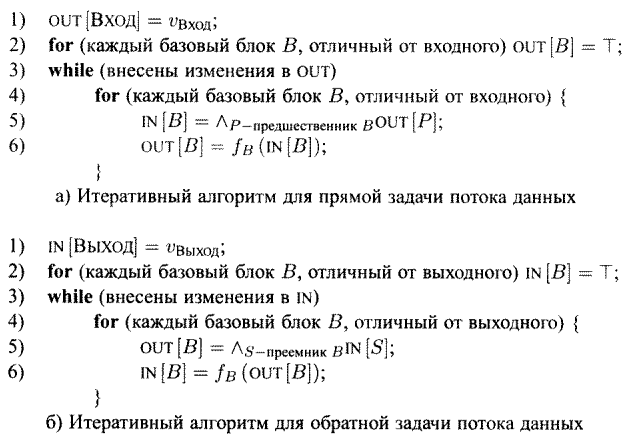
\includegraphics[width=0.8\columnwidth]{pics/dop26_iterative_algs.png}

Проходим по всем блокам и вычисляем множества In и Out для каждого блока пока что-то меняется. \textbf{\textbf{(Когда ничего не меняется это, видимо неподвижная точка, в драгонбуке называется фиксированной)}}

Для достигающих определений см. таблицу. Там еще есть другие анализы на всякий случай.

\begin{tabular}{|c|c|}
     \hline
     & Достигающие определения \\% & Активные переменные & Доступные выражения \\
     \hline
     \thead{Область \\ определения} & Множества определений \\%& Множества переменных & Множества выражений \\
     \hline
     Направление & Прямое \\ %&Обратное & Прямое \\
     \hline
     \thead{Передаточная \\ функция} & $gen_B \cup (x-kill_B)$\\%& $use_B \cup (x-def_B)$ & $e\_gen_B\cup(x-e\_kill_B)$ \\
     \hline
     \thead{Граничное \\ условие} & OUT[ВХОД] = $\emptyset$ \\%& IN[ВЫХОД]=$\emptyset$ & OUT[ВХОД] = $\emptyset$ \\
     \hline
     \thead{Оператор \\ сбора} $\wedge$ & $\cup$ \\%& $\cup$ & $\cap$ \\
     \hline
     Уравнения & \thead{$OUT[B] = f_B(IN[B])$ \\ $IN[B]= \wedge _{P\in pred_(B)} OUT[P]$} \\%& \thead{$IN[B] = f_B(OUT[B])$ \\ $OUT[B] = \wedge _{S\in succ(B)}IN[S]$} & \thead{$OUT[B] = f_B(IN[B])$ \\ $IN[B] = \wedge _{P\in pred_(B)} OUT[P]$} \\
     \hline
     Инициализация & OUT[B] = $\emptyset$ \\%& IN[B] = $\emptyset$ & OUT[B] = U \\
     \hline
\end{tabular}

% 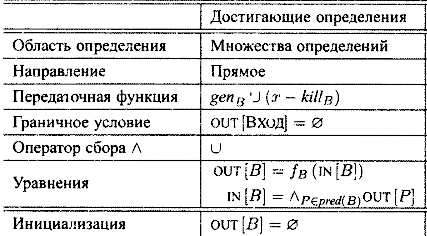
\includegraphics[width=0.65\columnwidth]{pics/dop26_analyzes.png}



% -------- source --------
\bigbreak
[\cite[9.2 - 9.3]{dragonbook}]